\icode{E-ME-SI-L3-261017-002}
如图所示，足够长的传送带倾角为 \(\theta\)，以恒定速率 \(v_1\) 沿顺时针方向传动。一物块从传送带顶端以沿传送带向下的初速度 \(v_2\) 滑上传送带，已知 \(v_2 > v_1\)，物块与传送带间的动摩擦因数 \(\mu\) 满足 \(\tan\theta < \mu\)。以物块刚滑上传送带的位置为位移起点，物块的动能 \(E_k\) 与位移 \(x\) 的关系图像可能正确的是\paren[]

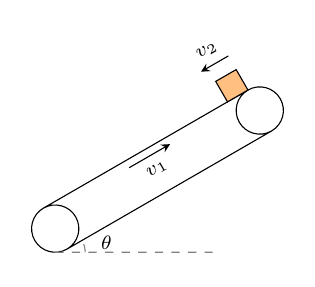
\begin{tikzpicture}[>=stealth,font=\scriptsize]
	\begin{scope}[rotate=30]
		\draw (0,0) circle(.3) (3,0) circle(.3) (0,.3)--(3,.3) (0,-.3)--(3,-.3);
		\draw[fill=orange!50] (3,.3) rectangle(2.7,.6);
		\draw[->] (3,.8)--node[above,rotate=30]{\(v_2\)}(2.6,.8);
		\draw[->] (1.2,.2)--node[below,rotate=30]{\(v_1\)}(1.8,.2);
	\end{scope}
	\draw[dashed,gray] (0,-.3)--(2,-.3) ({.3*tan(15)+.3},-.3) arc(0:30:.3);
	\node at(.65,-.18){\(\theta\)};
\end{tikzpicture}

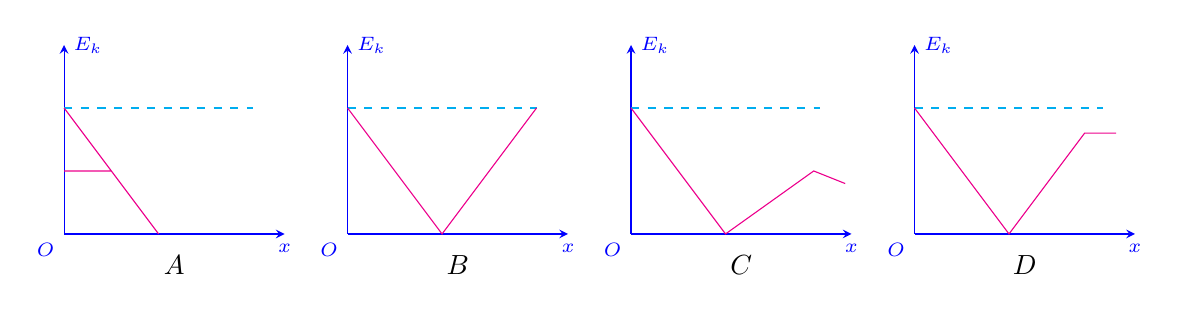
\begin{tikzpicture}[scale=.8,>=stealth,font=\scriptsize]
	\begin{scope}
		\draw[->,blue] (0,0)node[below left]{\(O\)}--(3.5,0)node[below]{\(x\)};
		\draw[->,blue] (0,0)--(0,3)node[right]{\(E_k\)};
		\draw[dashed,cyan] (0,2)--(3,2);
		\draw[magenta] (0,2)--(1.5,0) (0,1)--(.75,1);
		\node at(1.75,-.5){\normalsize\(A\)};
	\end{scope}
	\begin{scope}[xshift=4.5cm]
		\draw[->,blue] (0,0)node[below left]{\(O\)}--(3.5,0)node[below]{\(x\)};
		\draw[->,blue] (0,0)--(0,3)node[right]{\(E_k\)};
		\draw[dashed,cyan] (0,2)--(3,2);
		\draw[magenta] (0,2)--(1.5,0)--(3,2);
		\node at(1.75,-.5){\normalsize\(B\)};
	\end{scope}
	\begin{scope}[xshift=9cm]
		\draw[->,blue] (0,0)node[below left]{\(O\)}--(3.5,0)node[below]{\(x\)};
	    \draw[->,blue] (0,0)--(0,3)node[right]{\(E_k\)};
		\draw[dashed,cyan] (0,2)--(3,2);
		\draw[magenta] (0,2)--(1.5,0)--(2.9,1)--(3.4,.8);
		\node at(1.75,-.5){\normalsize\(C\)};
	\end{scope}
	\begin{scope}[xshift=13.5cm]
		\draw[->,blue] (0,0)node[below left]{\(O\)}--(3.5,0)node[below]{\(x\)};
		\draw[->,blue] (0,0)--(0,3)node[right]{\(E_k\)};
		\draw[dashed,cyan] (0,2)--(3,2);
		\draw[magenta] (0,2)--(1.5,0)--(2.7,1.6)--(3.2,1.6);
		\node at(1.75,-.5){\normalsize\(D\)};
	\end{scope}
\end{tikzpicture}
\begin{answer}
    A\qquad 提示：\(\frac{\Delta E_k}{\Delta x} = F\)
\end{answer}